\subsection{System Arkitektur}

\begin{frame}{Hardware Komponenter (1)}
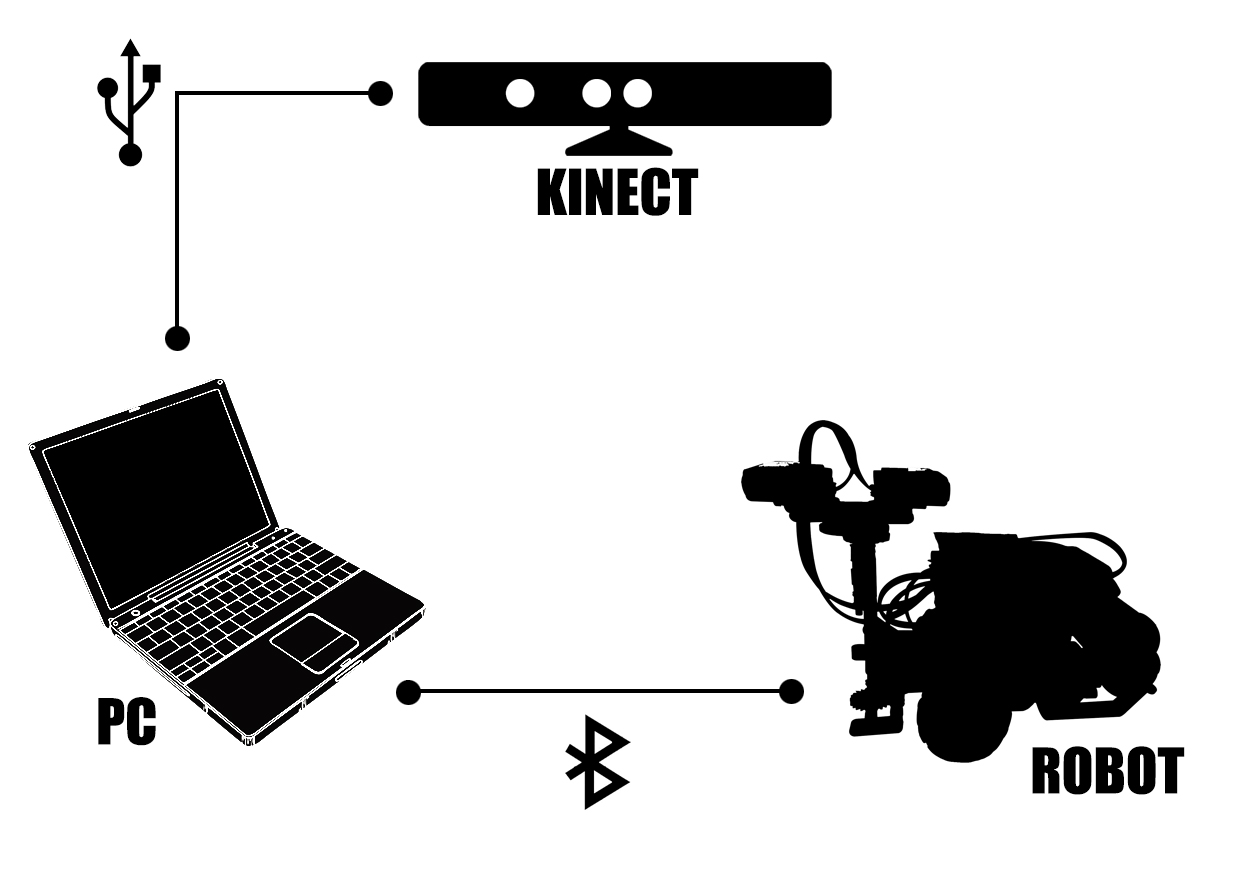
\includegraphics[width=\textwidth]{enheder}
\end{frame}

\begin{frame}{Hardware Komponenter (2)}
\begin{description}
\item[Kinect]{Billed-feed til lokalisering}
\item[NXT]{Navigation i/observation af verden}
\item[PC]{Beregning af:}
\begin{itemize}
\item{kort}
\item{robot lokation}
\item{rute}
\end{itemize}
\end{description}
\end{frame}

\begin{frame}{Hardware Komponenter (3)}
\begin{itemize}
\item{Proof of concept kontra anvendelighed;}
\begin{itemize}
\item{Mulighed for at isolere et enkelt problem}
\item{''Simulering'' af god lokationsberegning\\
samt højere regnekraft}
\end{itemize}
\item{Mulighed for udskiftning af komponent(er)}
\end{itemize}
\end{frame}

\subsection{NXT}

\begin{frame}{NXT Software}
3 overordnede filer, med hver deres funktionalitet:
\begin{description}
\item[Sensor.nxc]{Observation af verden}
\item[Navigation.nxc]{Navigation i verden}
\item[Communication.nxc]{Kommunikation med PC}
\end{description}
\end{frame}

\subsection{PC}

\begin{frame}{PC Software (1)}
Indsæt overordnet diagram (Yderste komponenter)
\end{frame}

\begin{frame}{PC Software (2)}
\begin{description}
\item[CommonLib]{DTOs, NXTPostMan, Interfaces}
\item[SystemInterface]{GUI og RobotInterface}
\item[Control]{Display, Location og Mapping}
\item[Services]{Robot, Route, Kinect, Tracking}
\item[Data]
\end{description}
\end{frame}

\subsection{Kommunikation}

